\chapter{Implementation Details} \label{implementationDetails}

\section{Introduction to AMBER and NEXMD}

NEXMD, currently being developed by the Tretiak lab in los Alamos, has a proven track record of performance on the stimulation of ultra-fast non-adiabatic behaviors.
It’s ability to solve state coupling equations on-the-fly has found great utility for systems with hundreds of atoms.
Numerous studies have implemented the method for research into topics including the study of chlorophyll organic conjugated molecules, and pi conjugated macrocycles. \cite{zheng2017photoinduced,nelson2014nonadiabatic,alfonso2016interference,wu2006exciton,Ondarse-Alvarez2016} 
Such studies with NEXMD have been limited to implicit solvents.
No method to provide NEXMD with QM/MM capabilities have yet to be implemented.

Amber is primarily known as a classical force-field molecular dynamics package.
It’s a massive project maintained by people across the globe that's been designed to work with very large systems ranging in the tens of thousands of atoms. \cite{case2020a}
Amber is capable of a huge range of simulations from replica exchange to study ph-dependent conformation chagnges to QM/MM umbrella sampling using nudge elastic bands. \cite{cruzeiro2020exploring, ghoreishi2019fast,sarkar2019ph}
Most importantly for this research, it has a proven track record of doing QM/MM solvent-solute simulations using periodic boundary conditions.

\section{Schematics}
\noindent
\begin{minipage}[c]{\textwidth}
  \centering
  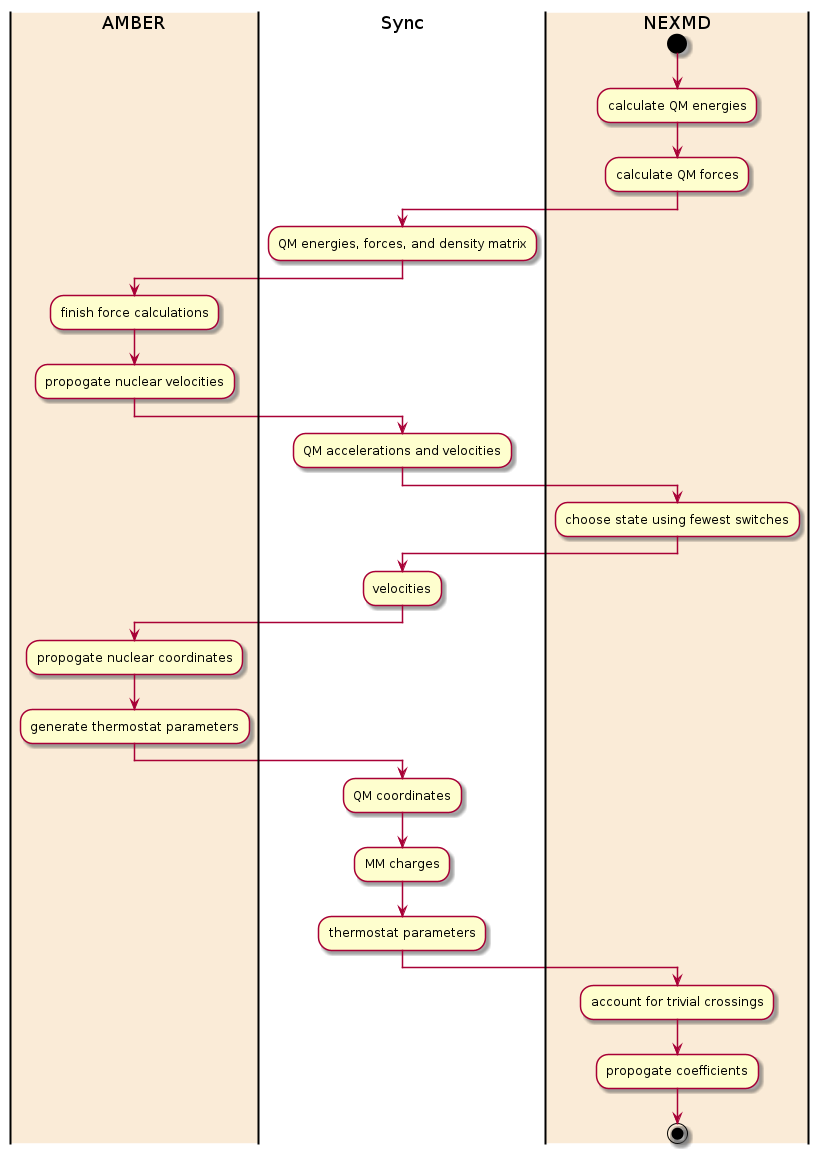
\includegraphics[width=0.5\linewidth]{../Paper2/scripted_diagrams/nasqm_overview.png}
  \captionof{figure}{Swim-lane diagram describing the common timestep of the SANDER-NEXMD interface.}
  \label{scheme:nasqm}
\end{minipage}\bigskip

The swim-lane chart in figure \ref{scheme:nasqm} describes a common time-step that occurs within the SANDER-NEXMD interface.
First users initiate the program through SANDER, a program found in AMBERTOOLS. SANDER uses NEXMD to calculate the energies and forces of the QM atoms, check for trivial crossings, and propagate the quantum coefficients.
With these results, SANDER performs the QM/MM procedures to derive the accelerations and velocities for the classical time step.
NEXMD then decides whether to perform a state transitions, adjusting the velocities as needed.
Finally SANDER propagates the nuclear coordinates and the cycle continues for the rest of the dynamics.

When users initiate SANDER, they're provide the usual SANDER inputs of a
coordinate, parameter, and sander control files.
In addition they will include a file specific to
NEXMD which describes the QM and Non-adiabatic behavior.
This interface, incorporates SANDER's implementation of QM/MM as described in previous literature to generate a solvent inclusive ground state density matrix utilized by NEXMD's excited state calculations.
Sander controls the interactions between the QM and MM regions.


SANDER calls NEXMD providing the function calls with the QM coordinates, MM charges, and Langevin thermostat parameters.\cite{paterlini1998constant}
NEXMD calculates the energies of the QM atoms with electrostatic interactions from the MM point charges using CIS, TDHF, or TDDFT.
A variety of Hamiltonians are available; however, AM1 has been shown to provide very reasonable computational cost to accuracy for our systems of interest.\cite{silva2010benchmark}
An analysis of parameter choices can be found in previous literature.\cite{nelson2012nonadiabatic}

We use SANDER's QM/MM implementation to provide approximations of the solvent interactions.\cite{Walker2008}
   SANDER's combined QM/MM Hamiltonian represents MM atoms as point charges and QM atoms as electronic wave-functions.
   The effective Hamiltonian uses the aforementioned hybrid approach
   \begin{equation}
     \mathbf{H}_{eff} = \mathbf{H}_{QM} + \mathbf{H}_{MM} + \mathbf{H}_{QM/MM}
   \end{equation}
   where \(\mathbf{H}_{QM}\), \(\mathbf{H}_{MM}\), \(\mathbf{H}_{QM/MM}\) are the Hamiltionians for the QM to QM, MM to MM, and QM to MM hybrid interactions.
   \(\mathbf{H}_{MM}\) is not considered during the electronic calculations due to it independence from the electronic distribution.
   \(\mathbf{H}_{QM}\) is the electronic Hamiltonian used in vacuum QM SCF calculations.
   \(\mathbf{H}_{QM/MM}\) represents the interactions between the QM charge density and MM atoms treated as point charges.
   For computational efficiency we limit the range of this interaction by a cuttoff, set by the user, generally in the range of 10-16 \(\AA\) from the paremeter QM atoms.
   For short range interactions the hybrid \(\mathbf{H}_{QM/MM}\) can be expanded into

   \begin{align}
     \mathbf{H}_{QM/MM} = &- \sum_i \sum_m q_m \hat{h}_{electron} (\vec{r}_i,  \vec{r}_m)\\
			  &+ \sum_q \sum_m q_q q_m \hat{h}_{core} (\vec{r}_q, \vec{r}_m)\\
			  &+ \sum_m \sum_q \left( \frac{A_{qm}}{r_{qm}^{12}} - \frac{B_{qm}}{r_{qm}^6} \right)
   \end{align}
   where \(i\) is the electron, \(m\) the MM atom, and \(q\) the combined nuclei and core electrons of the QM atoms.
   A and B are the Lennard-Jones interaction parameters where \(r_{qm}\) is the distance between the MM and QM atoms.
   \(q\) is the charge and \(r\) is the ccoordinate vector.
   \(\hat{h}_{core}\) represents the electronic interactions between the MM charges and the core of the QM atoms.
   \(\hat{h}_{electron}\) represents the interactions between the MM charges and either the charge density of the QM region when using Semi-emprical hamiltonians, or by using the Mulliken charges in the case of DFT.

   Long range interaction, from those outside the cutoff, considered vital for the understanding of solvent effects, are treated using SQM’s implementation of Particle Mesh Ewald.
   Trajectories use periodic boundary conditions to simulate an explicit solution, treating the system box as cells repeated infinitely many times in all directions.
   Particle Mesh Ewald calculations then determine the long-distance interactions of these periodic boxes, treating the charges and potentials in the long-range inter-box distances as sums in Fourier space treating atoms in the QM region of these calculations as Mulliken point charges.\cite{essman1995smooth}
   Once the sums are complete, SQM performs a fast Fourier transformation to obtain the long-range corrections to the energy and forces. 


   For a general timestep QM/MM interaction will be added to the density matrix as follows: 
\begin{enumerate}
   \item Calculate the MM ewald potentials using the classical charges from the MM atoms.
   \item Construct the Hamiltonian matrix as if the QM region was in vacuum.
   \item Add the one electron terms for the interaction between QM atoms and the MM atoms within the cutoff to the Hamiltonian.
   \item Within the SCF routine, copy the Hamiltonian to the fock matrix, and add the QM/MM two-electron integrals.
   \item Calculate the QM ewald potential using the iteration’s Mulliken charges, then add the ewald potentials for both QM and MM atoms to the Fock Matrix.
   \item The SCF procedure continues until convergence resulting in a density matrix that incorporates the presence of solvents. 
\end{enumerate}

Excited-state calculations implement the Collective Electronic Oscillator (CEO) approach developed by Mukamel and coworkers, which solves the adiabatic equation of motion of a single electron density matrix.\cite{Mukamel1997,tretiak02_densit_matrix_analy_simul_elect}
The single-electron density matrix is defined by
\begin{equation}
  (\rho_{g\alpha})_{nm} = \left< \psi_{\alpha} (t) \right| c_m^{\dagger} c_n \left| \psi_{g} (t) \right>
\end{equation}
where \(\psi_g\) and \(\psi_\alpha\) are the single-electron wave functions of the ground-state and \(\alpha\) state, and \(c_m^{\dagger} c_n\) is the creation(annihilation) operator summed over the atomic orbital \(m\) and \(n\), whose size is determined by the basis set.
The basis set coefficients of these atomic orbits are calculated in the previous SCF step and account for the presence of solvents.
The CIS approximation is applied, creating the normalization condition 

\begin{equation}
  \sum_{n,m} (\rho_{g\alpha})^2 = 1
\end{equation}

Recognizing that \(\rho_{g\alpha}\) represents the transition density from the ground to the \(\alpha\) state, we solve the Liouville equation of motion 

\begin{align*}
  \hat{\mathbf{\mathcal{L}}}\mathbf{\rho}_{0\alpha} = \Omega\mathbf{\rho}_{0\alpha}
\end{align*}


with \(\mathbf{\mathcal{L}}\) being the two-particle Louiville operator and
\(\Omega\) the energy difference between the \(\alpha\) state and the ground
state. \(\rho_{0\alpha}\) is the single- electron density matrix

\begin{align*}
  (\mathbf{\rho}_{0\alpha})_{nm} =  \left< \psi_{\alpha} \right| c_m^\dagger c_n \left| \psi_0 \right>.
\end{align*}
where \(\psi_{g}\) and \(\psi_{\alpha}\) are the single-electron wavefunctions for the groundstate and singly excited state \(\alpha\), and
\(c_m^\dagger\) and \(c_n\) are the creation and annihilation operator respectively. The coefficients for the atomic orbital basit sets are derived prior using the QM/MM methodology from the SQM package.\cite{Walker2008} The Liouville operator can be found analytically using 

\begin{align*}
  \hat{\mathbf{\mathcal{L}}}\mathbf{\rho}_{0\alpha} = \left[ \mathbf{F}^{\vec{R}}(\mathbf{\rho}_{00}), \mathbf{\rho}_{0\alpha} \right]
  + \left[ \mathbf{V}^{\vec{R}}(\mathbf{\rho}_{0\alpha}), \mathbf{\rho}_{00} \right]
\end{align*}

where \(\textbf{F}^{\vec{R}}\) is the Fock operator and \(\textbf{V}^{\vec{R}}\) is the column interchange operator.

The forces are also calculated analytically using the gradient of the ground state
energy and the excited state energy.

\begin{align*}
  \vec{\nabla} E_{\alpha} = \vec{\nabla} E_0 + \vec{\nabla} \Omega_{\alpha}
\end{align*}

With the gradient of the ground state being calculated by

\begin{align*}
  \vec{\nabla} E_0 = \frac{1}{2}\mathbf{Tr} \left[ \left( \mathbf{t}^{\vec{R}} + \mathbf{F}^{\vec{R}} \right) \mathbf{\rho}_{00} \right]
\end{align*}
where \(\textbf{t}\) is the single-electron kinetic operator.

The gradient of the excited state can derived using

\begin{align*}
  \vec{\nabla}\Omega_{\alpha} = \mathbf{Tr} \left[ \mathbf{F}^{\vec{R}} (\mathbf{\rho}_{\alpha\alpha} - \mathbf{\rho}_{00})\right]
  + \mathbf{Tr} \left[\mathbf{V}^{\vec{R}}\mathbf{\rho}_{0\alpha}^\dagger \mathbf{\rho}_{0\alpha} \right]
\end{align*}

where \(\mathbf{\rho}_{ij}\) represents the density or transition density matrix for states i and
j, \(\mathbf{F}\) is the Fock matrix and \(\mathbf{V}\) is the column interchange operator.

\begin{table}[H]
      \caption{Benchmark average timings for 0 to 1 excited states}
      \label{table:benchmarks1}
      % \begin{center}
      \begin{tabularx}{\textwidth}{XXXX}\hline
N States & N Solvent & Adiabatic (ms/step) & NonAdiatic (ms/step)\\\hline
0        & 0         &  1.34 & 2.89\\
0        & 1         &  2.35 & 4.32\\
0        & 3         &  3.14 & 8.85\\
0        & 5         &  5.89 & 10.42\\
0        & 10        & 11.87 & 13.32\\
0        & 15        & 16.34 & 19.81\\
1        & 0         &  1.34 & 25.22\\
1        & 1         &  2.35 & 29.12\\
1        & 3         &  3.14 & 32.98\\
1        & 5         &  5.89 & 36.01\\
1        & 10        & 11.87 & 40.33\\
1        & 15        & 16.34 & 45.63\\\hline
      \end{tabularx}
    \end{table}

    \begin{table}[H]
      \caption{Benchmark timings for 3 5, and 10 excited states}
      \label{table:benchmarks2}
      % \begin{center}
      \begin{tabularx}{\textwidth}{XXXX}\hline
N States & N Solvent & Adiabatic (ms/step) & NonAdiatic (ms/step)\\\hline
3        & 0         &  2.34 & 4.89\\
3        & 1         &  3.35 & 8.32\\
3        & 3         &  4.14 & 15.85\\
3        & 5         &  7.89 & 20.42\\
3        & 10        & 14.87 & 25.32\\
3        & 15        & 19.34 & 38.81\\
5        & 0         &  2.34 & 50.22\\
5        & 1         &  3.35 & 58.12\\
5        & 3         &  4.14 & 64.98\\
5        & 5         &  7.89 & 72.01\\
5        & 10        & 13.87 & 80.33\\
5        & 15        & 20.34 & 90.63\\
10        & 0         &  4.34 & 100.22\\
10        & 1         &  6.35 & 120.12\\
10        & 3         &  8.14 & 128.98\\
10        & 5         &  14.89 & 144.01\\
10        & 10        & 26.87 & 160.33\\
10        & 15        & 40.34 & 180.63\\\hline
      \end{tabularx}
    \end{table}

Figures \ref{table:benchmarks1} and \ref{table:benchmarks2} show the timings for the Sander-NEXMD interfaces. 
Benchmarks consisted of a single PPV\(_3\)-NO\(_2\) molecule surrounded by 3423 CCl\(_4\) molecules.
PPV\(_3\)-NO\(_2\) consistes of 50 atoms, and every additional CCL\l\(_4\) molecule adds an additional 5 atoms.
A various number of solvent molecules are included in the QM region as shown in the second column.
The adiabatic dynamics seems to increase on the order of O(3) for the number of solvents and O(1) for the number of states.
This coincides to what we expect from the precedures found in configuration interactions.
The order for the number solvents orresponds to what we expect using AM1 semi-empirical method.
For non-adiabatic dynamics, the computation time seems to increase on the order of O(3) for the number of solvents and O(2) for the number of states.
The computational order on the number of solvents does is near identical for to the adiabatic since the non-adiabatic dynamics perform the same AM1 calculations.
The time order in the number of states however, differs because of the time used to calculate the non-adiabatic coupling vector and terms.
